\documentclass[12pt, a4paper]{article}

% \usepackage{extsizes}  % 字體文件使用 14pt
\usepackage{xeCJK}
\usepackage[margin=2.0cm]{geometry}
\usepackage{fancyhdr}
\usepackage{graphicx}
\usepackage{amsmath, amssymb, amsfonts}
\usepackage{listings}  % code showing
\usepackage{pagecolor}  % code color define
\usepackage{tocloft}  % contents
\usepackage{booktabs}
\usepackage{bm}

% -- 字體 (注意檔案是否存在)
\setCJKmainfont{cwTeXKai}
\setmainfont{Times New Roman}

% -- 格式
\pagestyle{fancy}  % 使用 header
\fancyhf{}
\setcounter{secnumdepth}{-1}  % 移除 section 數字
\renewcommand{\cftsecleader}{\cftdotfill{\cftdotsep}}

%% -- 標題使用中文取代
\renewcommand{\figurename}{圖}
\renewcommand{\tablename}{表}
\renewcommand{\lstlistingname}{程式碼}

%% -- 間距設定
% \linespread{1.2}\selectfont  % 行距
\setlength{\headheight}{29pt}  % header 最低高度
\setlength{\parindent}{0pt}  % 取消縮排
\setlength{\parskip}{0.5em}  % 段落距離
\setlength{\abovecaptionskip}{10pt}  % 圖表標題 caption 與圖表的距離
\setlength{\belowcaptionskip}{10pt}

%% -- 顯示程式碼
\definecolor{codegreen}{rgb}{0,0.6,0}
\definecolor{codegray}{rgb}{0.5,0.5,0.5}
\definecolor{codepurple}{rgb}{0.58,0,0.82}
\definecolor{backcolour}{rgb}{0.95,0.95,0.92}
\lstdefinestyle{Matlab}{
    backgroundcolor=\color{backcolour},
    commentstyle=\color{codegreen},
    keywordstyle=\color{magenta},
    numberstyle=\footnotesize\color{codegray},
    stringstyle=\color{codepurple},
    basicstyle=\ttfamily\footnotesize,
    breakatwhitespace=false,
    breaklines=true,
    captionpos=b,
    keepspaces=true,
    numbers=left,
    numbersep=5pt,
    showspaces=false,
    showstringspaces=false,
    showtabs=false,
    tabsize=2,
    extendedchars=false
}
\lstset{style=Matlab}

% ---------------------------------------------
\begin{document}
\chead{\normalsize \textbf{Homework}}  % 可調整大小
\lhead{\normalsize 2021 SOLab Orientation}
\rhead{\normalsize R10522601 林易玄}
\cfoot{\thepage}
\tableofcontents\thispagestyle{fancy}

% ---------------------------------------------
\section{Problem : Ten-bar Truss Optimization}
十桿桁架 (ten-bar truss) 是典型的桁架結構之一,如圖 \ref{f:structure} 所示。請利用此十桿桁架範例,演示如何使用有限元素法解決桁架的問題,並最佳化桿件截面半徑。
\begin{figure}[h]
    \centering
    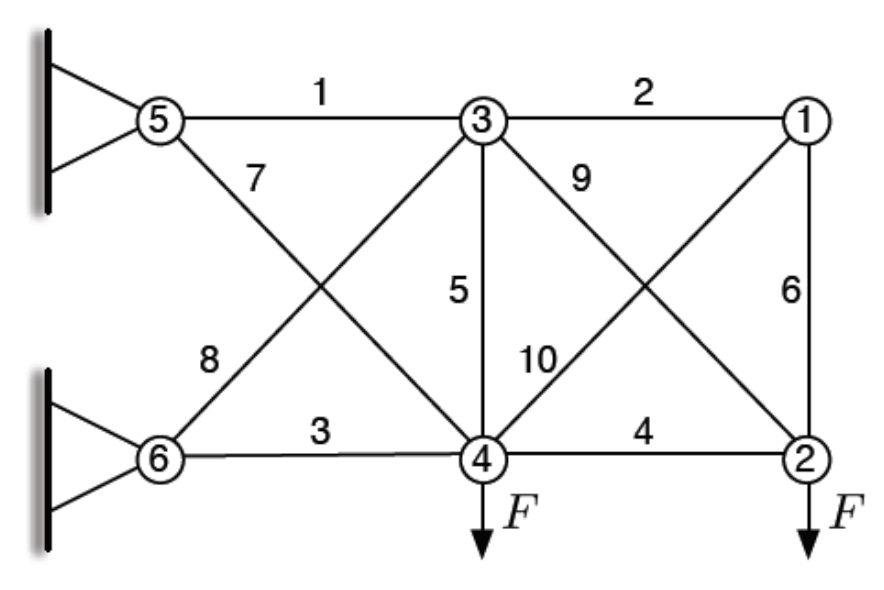
\includegraphics[width=12cm]{./pic/ten bar truss}
    \caption{Ten-bar truss 結構示意圖}
    \label{f:structure}
\end{figure}

\subsection*{Problem Definition}
在以下的已知條件下,給定桿件截面半徑,試求各桿件的位移、應力與反作用力:
\begin{itemize}
    \item 整體架構處在靜力平衡的情況下
    \item 所有桿件截面皆為圓形
    \item 材料為鋼,楊氏係數 E = 200 GPa,密度 $\rho$ = 7860 kg/m$^3$,降伏強度 $\sigma_y$ = 250 MPa
    \item 平行桿件與鉛直桿件(桿件1至桿件6)長度皆為 9.14 m
    \item 桿件 1 至桿件 6 截面半徑相同為 $r_1$,桿件 7 至桿件 10 截面半徑相同為 $r_2$
    \item 所有桿件半徑的最佳化範圍為 0.001 至 0.5 m 之間
    \item 在節點 2 和節點 4 上的負載 F 皆為 1.0 × 10$^7$ N 向下
\end{itemize}

\subsection*{Solution}
\begin{enumerate}
    \item 最佳化數學表示式:
    \begin{align}
        \begin{split}
            \min_{r_1,r_2} \quad & f(r_1,r_2) = \sum_{i=1}^{6} m_i(r_1) + \sum_{i=7}^{10} m_i(r_2) \\
            \mbox{subject to} \quad & \left \lvert \bm{\sigma_i} \right \lvert \le \sigma_y\\
            & \Delta s_2 \le 0.02\\
            \mbox{where} \quad & f \mbox{:所有桿件的質量}\\
            & \Delta s_2 \mbox{:node 2 的位移}\\
            & \sigma_y \mbox{:降伏應力}\\
            & \bm{\sigma_i} \mbox{:所有桿件的應力}\\
        \end{split}
        \label{eq:opt}
    \end{align}
    
    \item 利用有限元素法分析 10-bar truss problem:
    
    將有限元素法應用在桁架,各桿件視為元素 (element)、元素間的連接為節點 (node),求解流程如圖 2。首先建立元素表格 (element table),利用表格中的資料計算出剛性矩陣 (stiffness matrix),再以力、剛性和位移三者之間的關係找出所求的位移,最後應力和反作用力也能透過位移計算而得。以下使用有限元素法原理計算,運算的過程將利用 Matlab 軟體輔助,撰寫成程式執行。
    \begin{figure}[h]
        \centering
        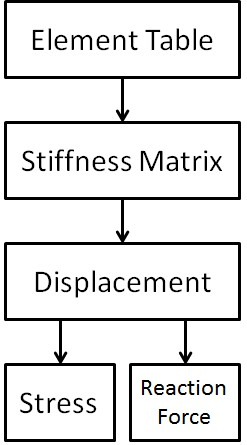
\includegraphics[width=4cm]{./pic/flowchart}
        \caption{計算流程圖}
        \label{f:flowchart}
    \end{figure}
    
    \begin{description}
        \item [Step 1] Element Table
        
        根據圖 \ref{f:structure} 與題目資訊,利用 Excel 製作表 \ref{t_1}、\ref{t_2}、\ref{t_3},提供 Matlab 在程式中讀取,如程式碼 \ref{code:data}。其中桿長與對應的三角函數計算方式如公式 \ref{eq:Length}、\ref{eq:cos}、\ref{eq:sin} 所示:
        
        \begin{equation}
            L = \sqrt{(x_{node \, j}-x_{node \, i})^2 + (y_{node \, j}-y_{node \, i})^2}
            \label{eq:Length}
        \end{equation}
        
        \begin{equation}
            \cos \theta_e = \frac{(x_{node \, j}-x_{node \, i})}{L}
            \label{eq:cos}
        \end{equation}
        
        \begin{equation}
            \sin \theta_e = \frac{(y_{node \, j}-y_{node \, i})}{L}
            \label{eq:sin}
        \end{equation}
        
        \begin{table}[!h]
    		\caption{節點座標 (node coordinate)}
    		\label{t_1}
    		\centering
    		\begin{tabular}{ccc}
        		\toprule
        		node & x & y\\
        		\midrule
        		1 & 18.28 & 9.14 \\
        		2 & 18.28 & 0 \\
        		3 & 9.14 & 9.14 \\
        		4 & 9.14 & 0 \\
        		5 & 0 & 9.14 \\
        		6 & 0 & 0 \\
        		\bottomrule
    		\end{tabular}
	    \end{table}
	    
        \begin{table}[!h]
    		\caption{元素表格 (element connectivity)}
    		\label{t_2}
    		\centering
    		\begin{tabular}{ccc}
        		\toprule
        		Element & node \textit{i} & node \textit{j}\\
        		\midrule
        		1 & 3 & 5 \\
        		2 & 1 & 3 \\
        		3 & 4 & 6 \\
        		4 & 2 & 4 \\
        		5 & 3 & 4 \\
        		6 & 1 & 2 \\
        		7 & 4 & 5 \\
        		8 & 3 & 6 \\
        		9 & 2 & 3 \\
        		10 & 1 & 4 \\
        		\bottomrule
    		\end{tabular}
	    \end{table}
	    
	    \begin{table}[!h]
    		\caption{節點負載 (load)}
    		\label{t_3}
    		\centering
    		\begin{tabular}{ccc}
        		\toprule
        		node & $F_x$ & $F_y$\\
        		\midrule
        		2 & 0 & $-1.0 × 10^7$ \\
        		4 & 0 & $-1.0 × 10^7$ \\
        		\bottomrule
    		\end{tabular}
	    \end{table}
        
        \lstinputlisting[
            language=Matlab, firstline=4, lastline=14, firstnumber=4,
            caption={資料讀取與參數設定}, label={code:data}
        ]{./FEMcon.m}
        
        \clearpage
        
        \item [Step 2] Stiffness Matrix
        
        每個元素末端連接兩個節點,節點又分別有 $x$ 和 $y$ 兩個方向的自由度 (degree of freedom,DOF),以 4 × 4 的剛性矩陣 (stiffness matrix,數學式中以 \textbf{k} 表示) 表示元素中 4 個自由度上位移和受力之間的相互關係:
        
        \begin{equation}
            \bm{k}^e = \frac{EA_e}{L_e}
            \left[
            \begin{array}{cccc}
                c^2 & cs & -c^2 & -cs\\
                cs & s^2 & -cs & -s^2\\
                -c^2 & -cs & c^2 & cs\\
                -cs & -s^2 & cs & s^2
            \end{array}
            \right]
            \label{eq:klocal}
        \end{equation}\\
        其中 $c$ 表示$\cos \theta_e$;$s$ 表示 $\sin \theta_e$。
        
        桁架整體結構中有 6 個節點,總共有 2 × 6 = 12 個自由度,以 node1 在 $x$ 方向為 DOF1、 node1 在 $y$ 方向為 DOF2、node2 的 $x$ 方向為 DOF3......依 node1 到 node6 的順序和 $x$、$y$ 的順序編號 12 個自由度。透過元素表格揭露的數據代入式 \ref{eq:klocal},下方程式碼 \ref{code:klocal} 將展示 local stiffness matrix 的計算:
        
        \lstinputlisting[
            language=Matlab, firstline=16, lastline=51, firstnumber=16,
            caption={Local Stiffness Matrix}, label={code:klocal}
        ]{./FEMcon.m}
        
        \clearpage
        
        10 個元素皆參考元素表格代入式 \ref{eq:klocal} 推導出剛性矩陣後,按照所對應的自由度,整合成 12 × 12 的整體剛性矩陣 \textbf{K}:
        
        \begin{equation}
            \bm{K} \leftarrow \sum_{e} \bm{k}^e
            \label{eq:kglobal}
        \end{equation}
        
        下方程式碼 \ref{code:kglobal} 將展示 local 轉換成 global stiffness matrix 的方法,並一併計算節點負載的 force vector:
        
        \lstinputlisting[
            language=Matlab, firstline=53, lastline=77, firstnumber=53,
            caption={Global Stiffness Matrix and Force Vector}, label={code:kglobal}
        ]{./FEMcon.m}
        
        \item [Step 3] Displacement
        
        利用 \textbf{Step 2} 中求得的力與剛性,將可求得位移,其三者關係如式 \ref{eq:F=Kd}:

        \begin{equation}
            \left[
            \begin{array}{c}
                F_1\\
                F_2\\
                \vdots\\
                F_{12}
            \end{array}
            \right]
            =
            \left[
            \begin{array}{cccc}
                K_{1,1} &K_{1,2} &\dotso &K_{1,12}\\
                K_{2,1} &K_{2,2} &\dotso &K_{2,12}\\
                \vdots &\vdots &\ddots &\vdots\\
                K_{12,1} &K_{12,2} &\dotso &K_{12,12}
            \end{array}
            \right]
            \cdot
            \left[
            \begin{array}{c}
                d_1\\
                d_2\\
                \vdots\\
                d_{12}
            \end{array}
            \right]
            \label{eq:F=Kd}
        \end{equation}\\
        其中必須考慮到邊界條件,由於 node5 和 node6 為固定端,因此位移為零,即 $d_9$ 至 $d_{12}$ 等於零,而在運算時也只需考慮 \textbf{K} 矩陣的前八行與列、\textbf{F} 向量的前八列,化簡矩陣程式碼如 \ref{code:bc} 所示,而利用式 \ref{eq:F=Kd} 將可求得各節點位移,並最後補上邊界條件的位移,其程式碼如 \ref{code:disp} 所式:
        
        \clearpage
        
        \lstinputlisting[
            language=Matlab, firstline=79, lastline=88, firstnumber=79,
            caption={矩陣去除邊界條件}, label={code:bc}
        ]{./FEMcon.m}
        
        \lstinputlisting[
            language=Matlab, firstline=90, lastline=93, firstnumber=90,
            caption={節點位移計算}, label={code:disp}
        ]{./FEMcon.m}
        
        \item [Step 4] Stress and Reaction Force
        
        應力與應變的關係如下:
        
        \begin{equation}
            \sigma = E \times \varepsilon
            \label{eq:stress}
        \end{equation}\\
        其中,$\sigma$ 為應力;$\varepsilon$ 為應變;$E$ 為楊氏係數。
        
        應變的定義為:
        
        \begin{equation}
            \varepsilon = \frac{\delta}{L}
            \label{eq:strain}
        \end{equation}\\
        其中,$\delta$ 為長度變量。
        
        元素的長度變量可以透過節點在各方向的位移作三角函數的轉換得到:
        
        \begin{equation}
            \bm{\sigma} = \frac{E_e}{l_e} 
            \left[
            \begin{array}{cccc}
                -c &-s &c &s\\ 
            \end{array}
            \right]
            \bm{d}
            \label{eq:stress2}
        \end{equation}
        
        而利用式 \ref{eq:stress2},將可求得各應力,而反作用力亦可從式 \ref{eq:F=Kd} 求得,其程式碼如 \ref{code:stressandreaction} 所式:
        
        \lstinputlisting[
            language=Matlab, firstline=95, lastline=107, firstnumber=95,
            caption={元素應力與節點反作用力計算}, label={code:stressandreaction}
        ]{./FEMcon.m}
    
    \end{description}

    \item 使用 fmincon 進行最佳化:
    
    使用 fmincon 函式進行最佳化時,程式檔案包括 Main 、 Objection 、 Constraints 三個檔案,本專案分別命名為 main.m 、 FEMobj.m 、 FEMcon.m,其中為符合 fmincon 的輸入型式,須先將最佳化數學式轉換為 negative null form,如式 \ref{eq:opt2} 所示:
    \begin{align}
        \begin{split}
            \min_{r_1,r_2} \quad & f(r_1,r_2) = \sum_{i=1}^{6} m_i(r_1) + \sum_{i=7}^{10} m_i(r_2) \\
            \mbox{subject to} \quad & \left \lvert \bm{\sigma_i} \right \lvert - \sigma_y \le 0 \\
            & \Delta s_2 - 0.02 \le 0\\
        \end{split}
        \label{eq:opt2}
    \end{align}\\
    由於 constrains 式會使用到 FEM 的計算結果,因此上方提及的程式碼 \ref{code:data} 至 \ref{code:stressandreaction} 皆是撰寫在 FEMcon.m 中,而 constrains 撰寫與整體 FEMcon.m 檔案 function 格式如程式碼 \ref{code:con} 所示:
    
    \lstinputlisting[
        language=Matlab, firstline=1, lastline=2,     firstnumber=1,
    ]{./FEMcon.m}
    
    \lstinputlisting[
        language=Matlab, firstline=109, lastline=115,     firstnumber=109,
        caption={Constraints function}, label={code:con}
    ]{./FEMcon.m}
    
    該題目目標為桿件最小總質量,利用截面積、桿長與材料密度來計算桿件質量,再根據目標函數公式 \ref{eq:opt2} 撰寫 FEMobj.m,如程式碼 \ref{code:obj} 所示:
    
    \lstinputlisting[
        language=Matlab,
        caption={Objection function}, label={code:obj}
    ]{./FEMobj.m}
    
    最後給定主程式桿件長度範圍與起始點,利用 fmincon 函式並呼叫撰寫完成的 FEMcon、FEMobj 來運算。main.m 撰寫如程式碼 \ref{code:main} 所示:
    
    \lstinputlisting[
        language=Matlab,
        caption={Main function}, label={code:main}
    ]{./main.m}
    
    根據程式執行結果,可得其最佳值與最佳解:
    
    \begin{displaymath}
        (r_1,r_2) = (0.2937,0.2665) \quad f = 207470
    \end{displaymath}\\
    此結果代表在桿件 1 至桿件 6 截面半徑為 0.2937 m,桿件 7 至桿件 10 截面半徑為 0.2665 m 時,得到其最小總質量為 207470 kg,且此設計符合安全規範。其目標函數值與疊帶次數關係如下圖 \ref{f:result}:
    
    \begin{figure}[h]
        \centering
        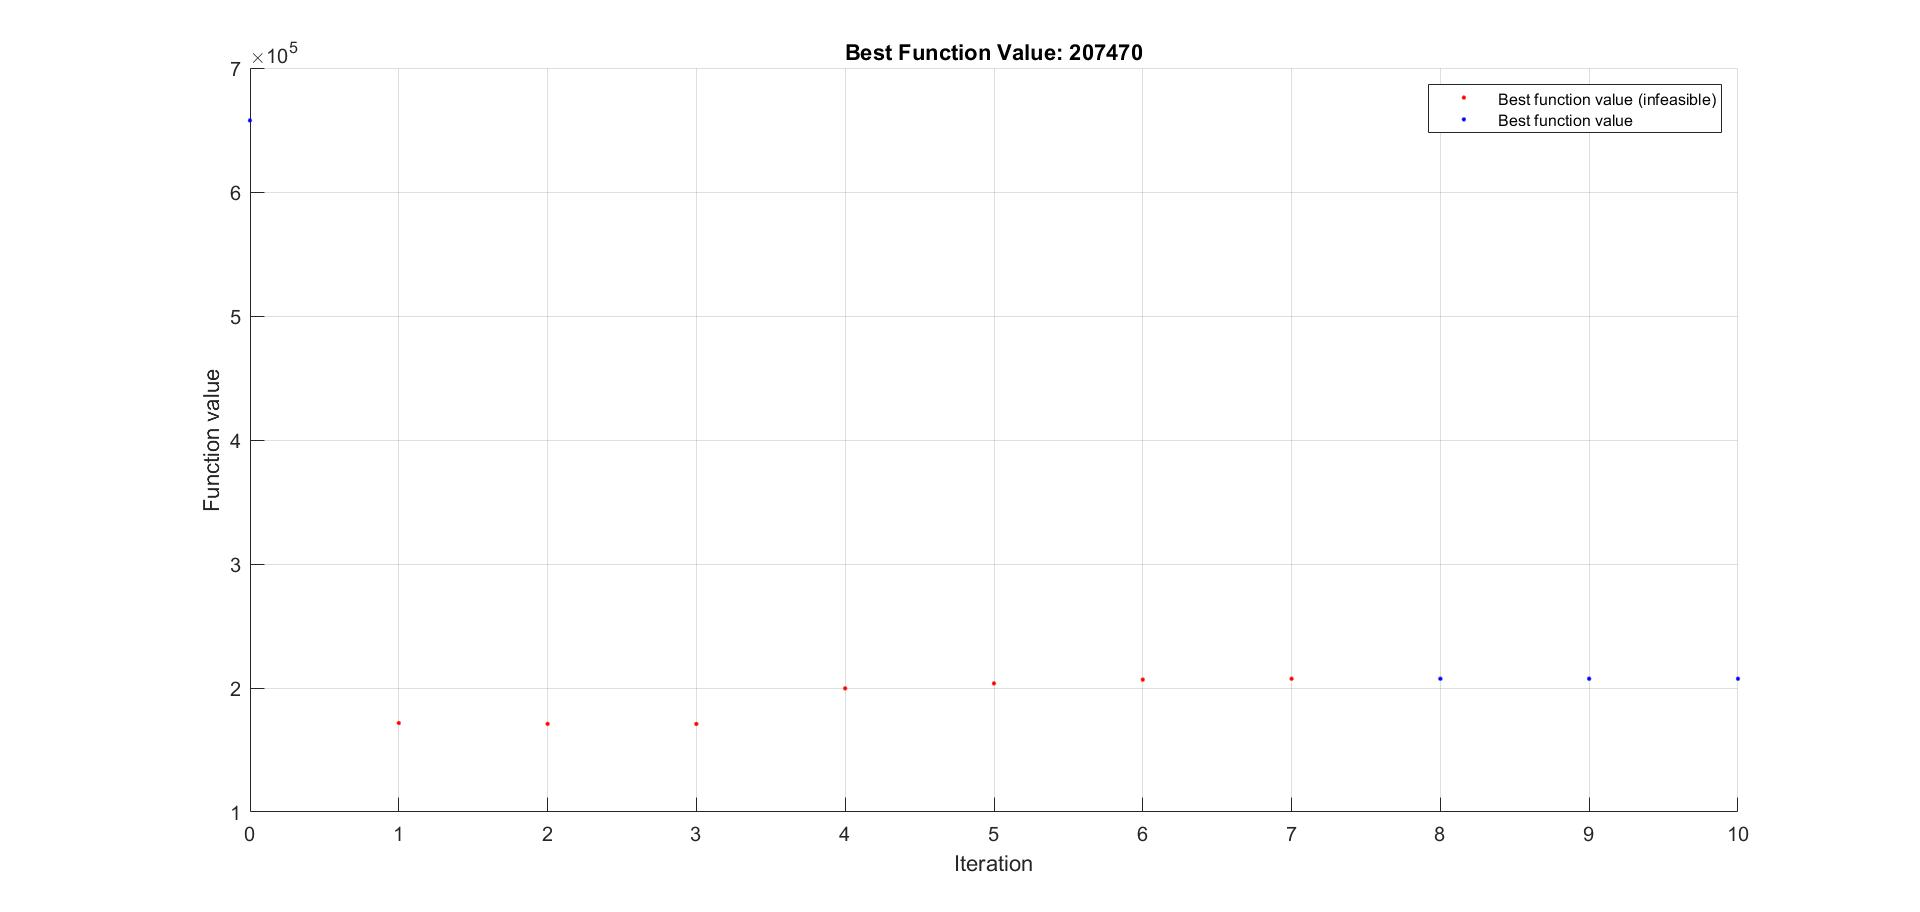
\includegraphics[width=17cm]{./pic/result}
        \caption{目標函數值與疊帶次數關係圖}
        \label{f:result}
    \end{figure}
    
\end{enumerate}
\clearpage

% ---------------------------------------------
\begin{thebibliography}{}
    \bibitem{manual} 
    SOLab.  
    \textit{SOLab\_manual\_v1.3.pdf}
    \bibitem{fem} 
    SOLab. 
    \textit{Finite Element Truss.pdf}
\end{thebibliography}

\end{document}
